\documentclass[11pt]{article}


\usepackage{fullpage}
\usepackage{graphicx}
\usepackage{amsmath}
\usepackage{amssymb}
\usepackage{amsthm}
\usepackage{fancyvrb}

\newcommand{\myname}{Mehshan Mustafa}

\newenvironment{theorem}[2][Theorem]{\begin{trivlist}
\item[\hskip \labelsep {\bfseries #1}\hskip \labelsep {\bfseries #2.}]}{\end{trivlist}}
\newenvironment{lemma}[2][Lemma]{\begin{trivlist}
\item[\hskip \labelsep {\bfseries #1}\hskip \labelsep {\bfseries #2.}]}{\end{trivlist}}
\newenvironment{exercise}[2][Exercise]{\begin{trivlist}
\item[\hskip \labelsep {\bfseries #1}\hskip \labelsep {\bfseries #2.}]}{\end{trivlist}}
\newenvironment{problem}[2][Problem]{\begin{trivlist}
\item[\hskip \labelsep {\bfseries #1}\hskip \labelsep {\bfseries #2.}]}{\end{trivlist}}
\newenvironment{question}[2][Question]{\begin{trivlist}
\item[\hskip \labelsep {\bfseries #1}\hskip \labelsep {\bfseries #2.}]}{\end{trivlist}}
\newenvironment{corollary}[2][Corollary]{\begin{trivlist}
\item[\hskip \labelsep {\bfseries #1}\hskip \labelsep {\bfseries #2.}]}{\end{trivlist}}
\newenvironment{solution}{\begin{proof}[Solution]}{\end{proof}}
\newenvironment{idea}[2][Proof Idea.]{\textit{#1} #2}



\parindent0in
\pagestyle{plain}
\thispagestyle{plain}

\usepackage{csquotes}
\usepackage[shortlabels]{enumitem}

\newcommand{\dated}{\today}

\begin{document}

\textbf{Introduction to the Theory of
Computation}\hfill\textbf{\myname}\\[0.01in]
\textbf{Chapter 1: Regular Languages}\hfill\textbf{\dated}\\
\smallskip\hrule\bigskip

\begin{problem}{1.41}
For languages $A$ and $B$, let the perfect shuffle of $A$ and $B$ be the language
\[
\{w \ | \ w = a_{1}b_{1} \cdots a_{k}b_{k}, \ where \ a_{1} \cdots a_{k} \in A \ and \ b_{1} \cdots b_{k} \in B, \ each \ a_{i}, b_{i} \in \Sigma\}.
\]
Show that the class of regular languages is closed under perfect shuffle.
\end{problem}

\begin{proof}
Let $A$ and $B$ be regular languages recognized by corresponding DFAs $M$ and $N$. To show that the class of regular languages is closed under perfect shuffle, we give construction of an all-NFA $D$ that recognizes the perfect shuffle of $A$ and $B$.

\begin{center}
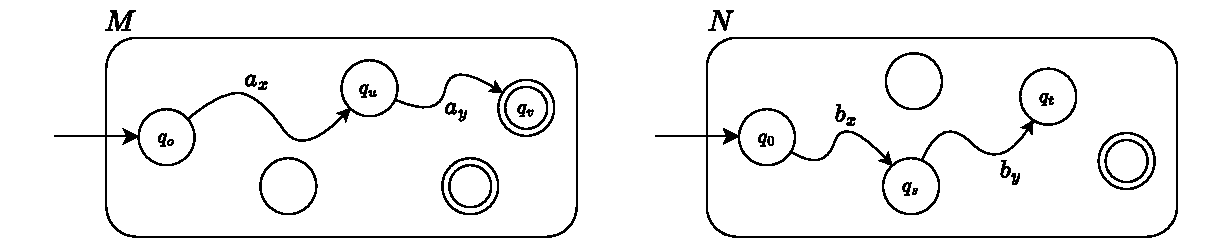
\includegraphics[scale=0.80]{Figures/Problem1.41a.pdf} \\
DFAs $M$ and $N$ recognize regular language $A$ and $B$ respectively. \\
$a_x, a_y, b_x, b_y \in \Sigma$.
\end{center}

\begin{center}
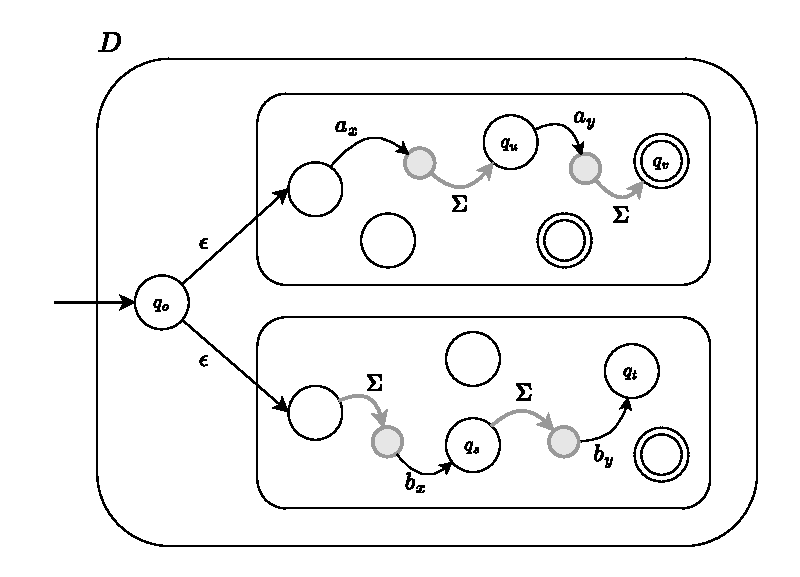
\includegraphics[scale=0.90]{Figures/Problem1.41b.pdf} \\
$D$ is an all-NFA that recognizes the the perfect shuffle of $A$ and $B$.
\end{center}

\end{proof}

\end{document}